\chapter{Results and Comparative Analysis}

\section{Phase 1 Classification Results}
The Phase 1 CNN achieved 53.94\% accuracy on the held-out test set of 33,000
RadioML examples, with a best validation accuracy of 54.02\%. Its accuracy
increased from 9.24\% at -20 dB SNR to 81.68\% at +12 dB SNR. This confirms
that the network learns modulation-dependent structure, while the low-SNR
performance shows the difficulty of recognizing heavily corrupted signals.

\begin{figure}[H]
\centering
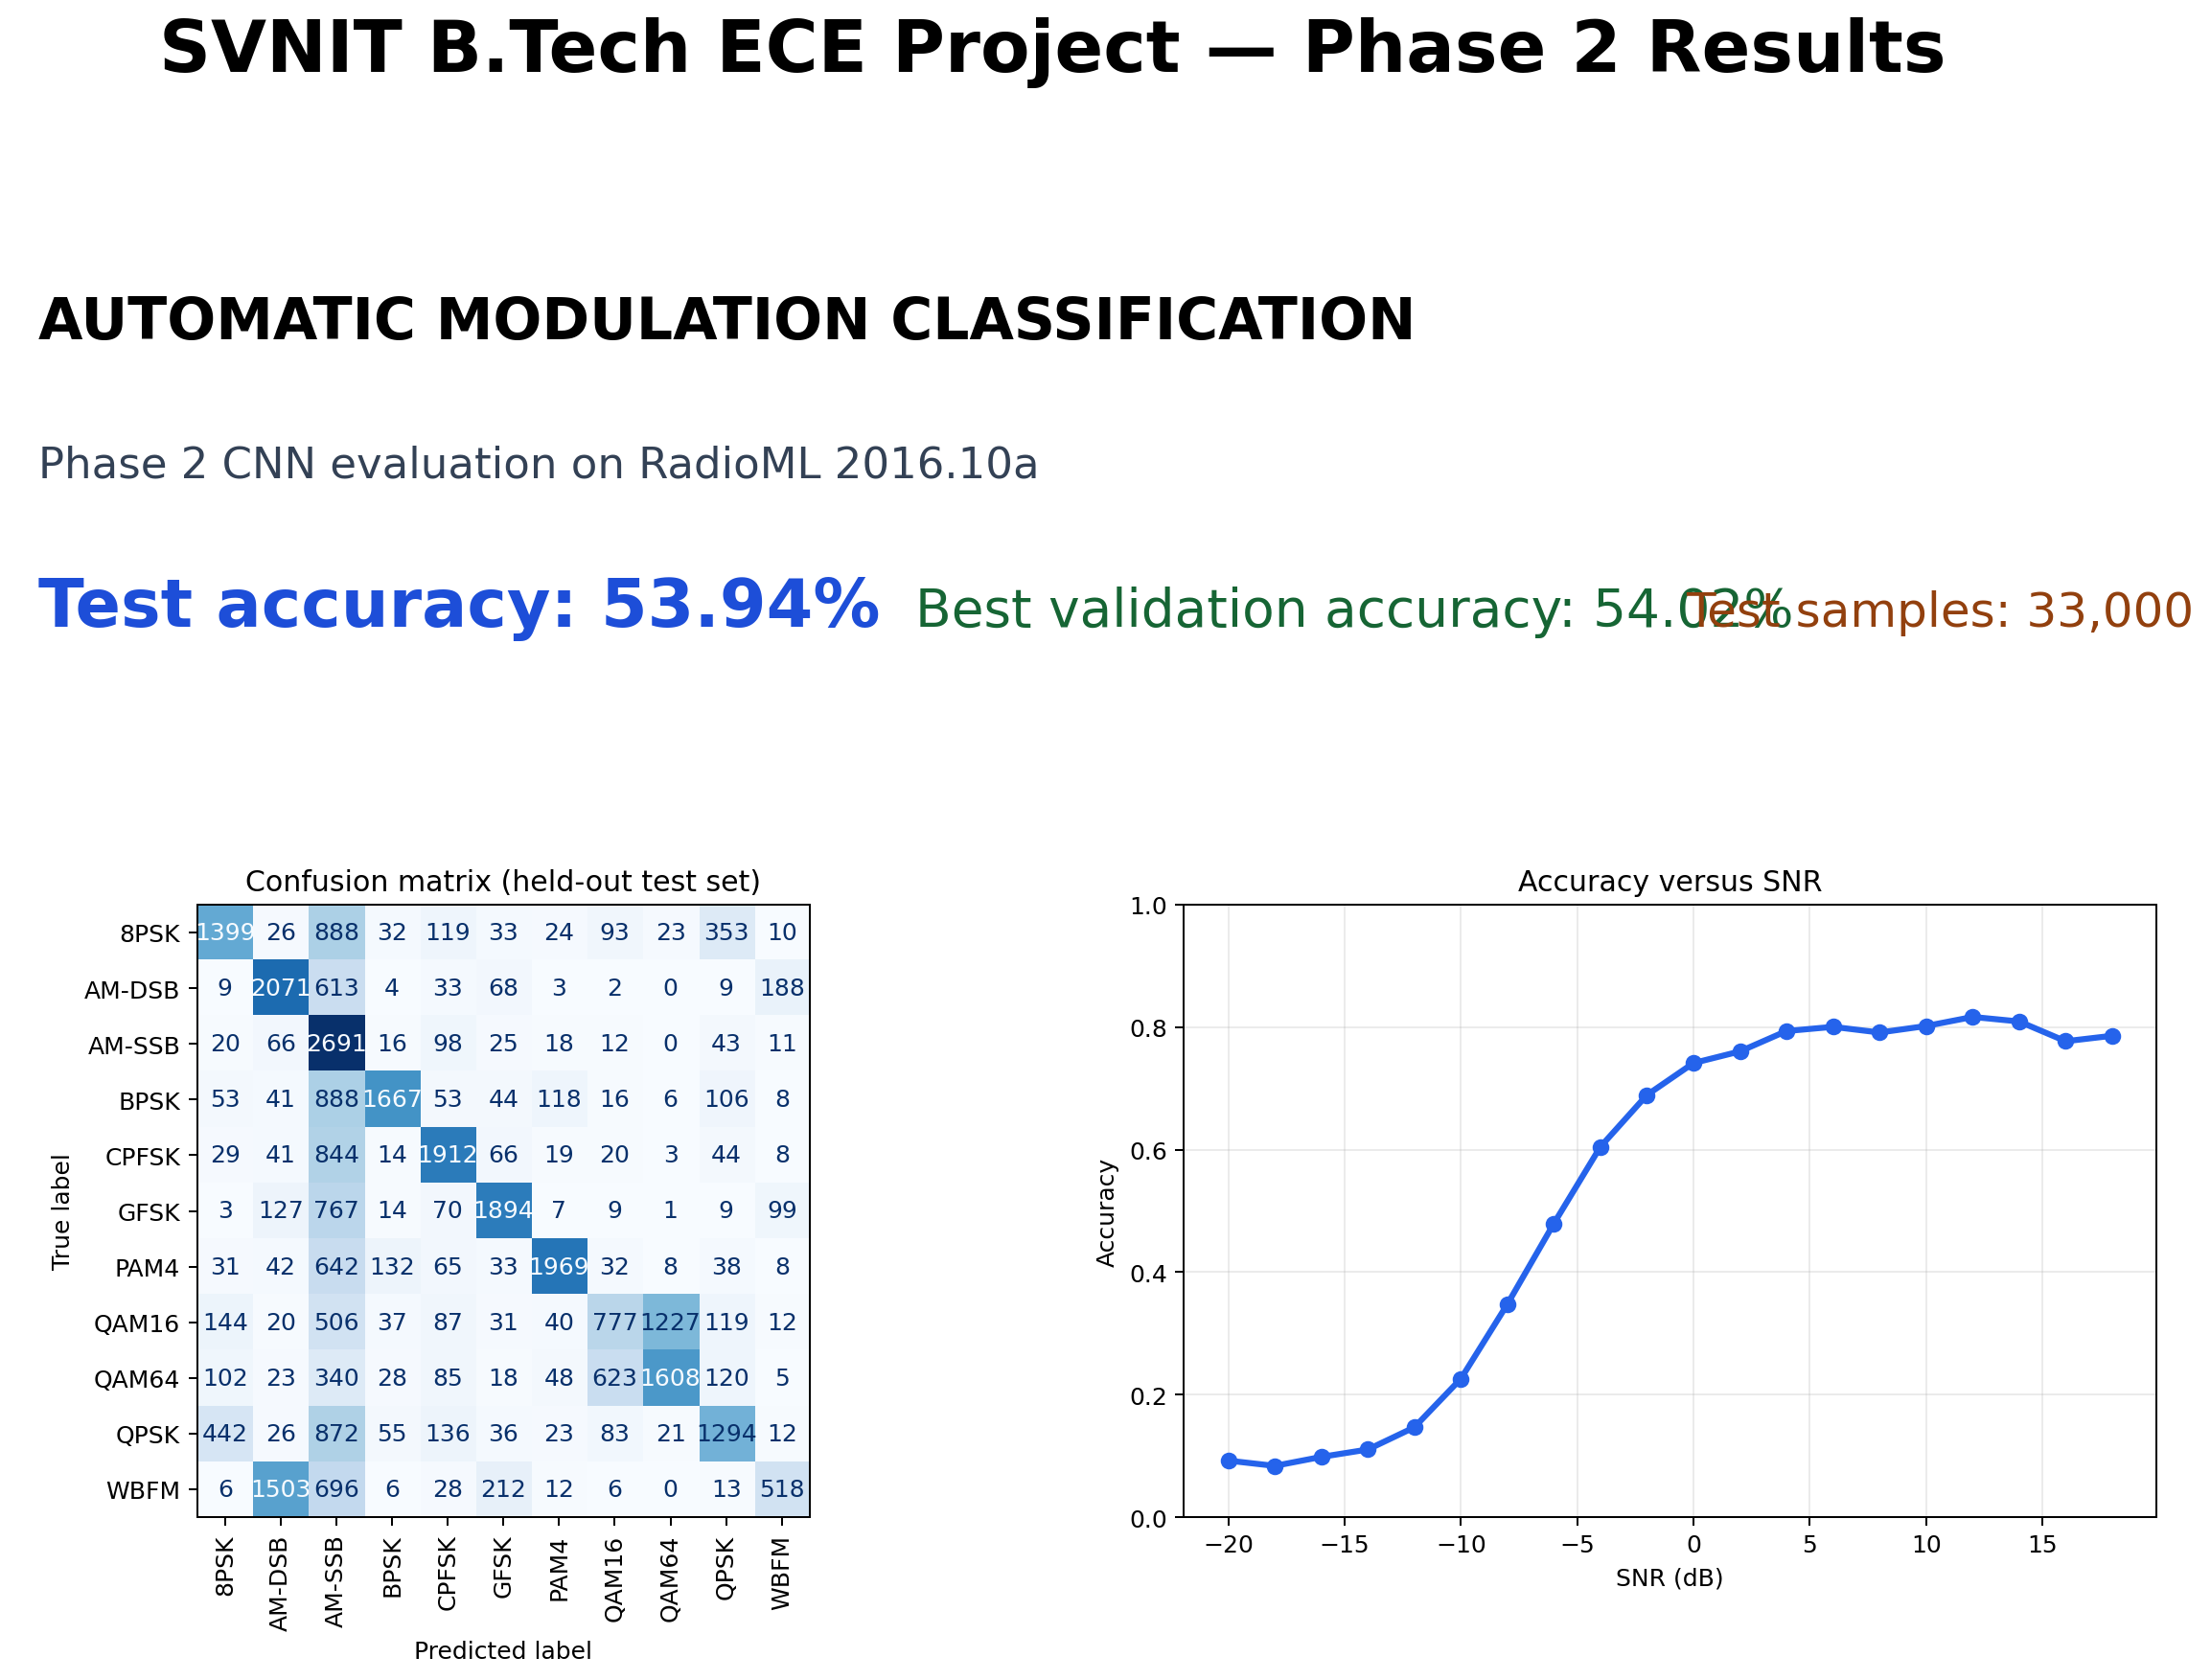
\includegraphics[width=\textwidth]{artifacts/phase2-results.png}
\caption{Phase 1 confusion matrix and SNR-wise accuracy.}
\label{fig:phase1result}
\end{figure}

\section{Phase 1 Training Behavior}
The validation history reaches its best reported value near the end of the
eight-epoch run. The checkpoint stores the history so that the plotted curve
can be reproduced without manually entering values.

\begin{figure}[H]
\centering
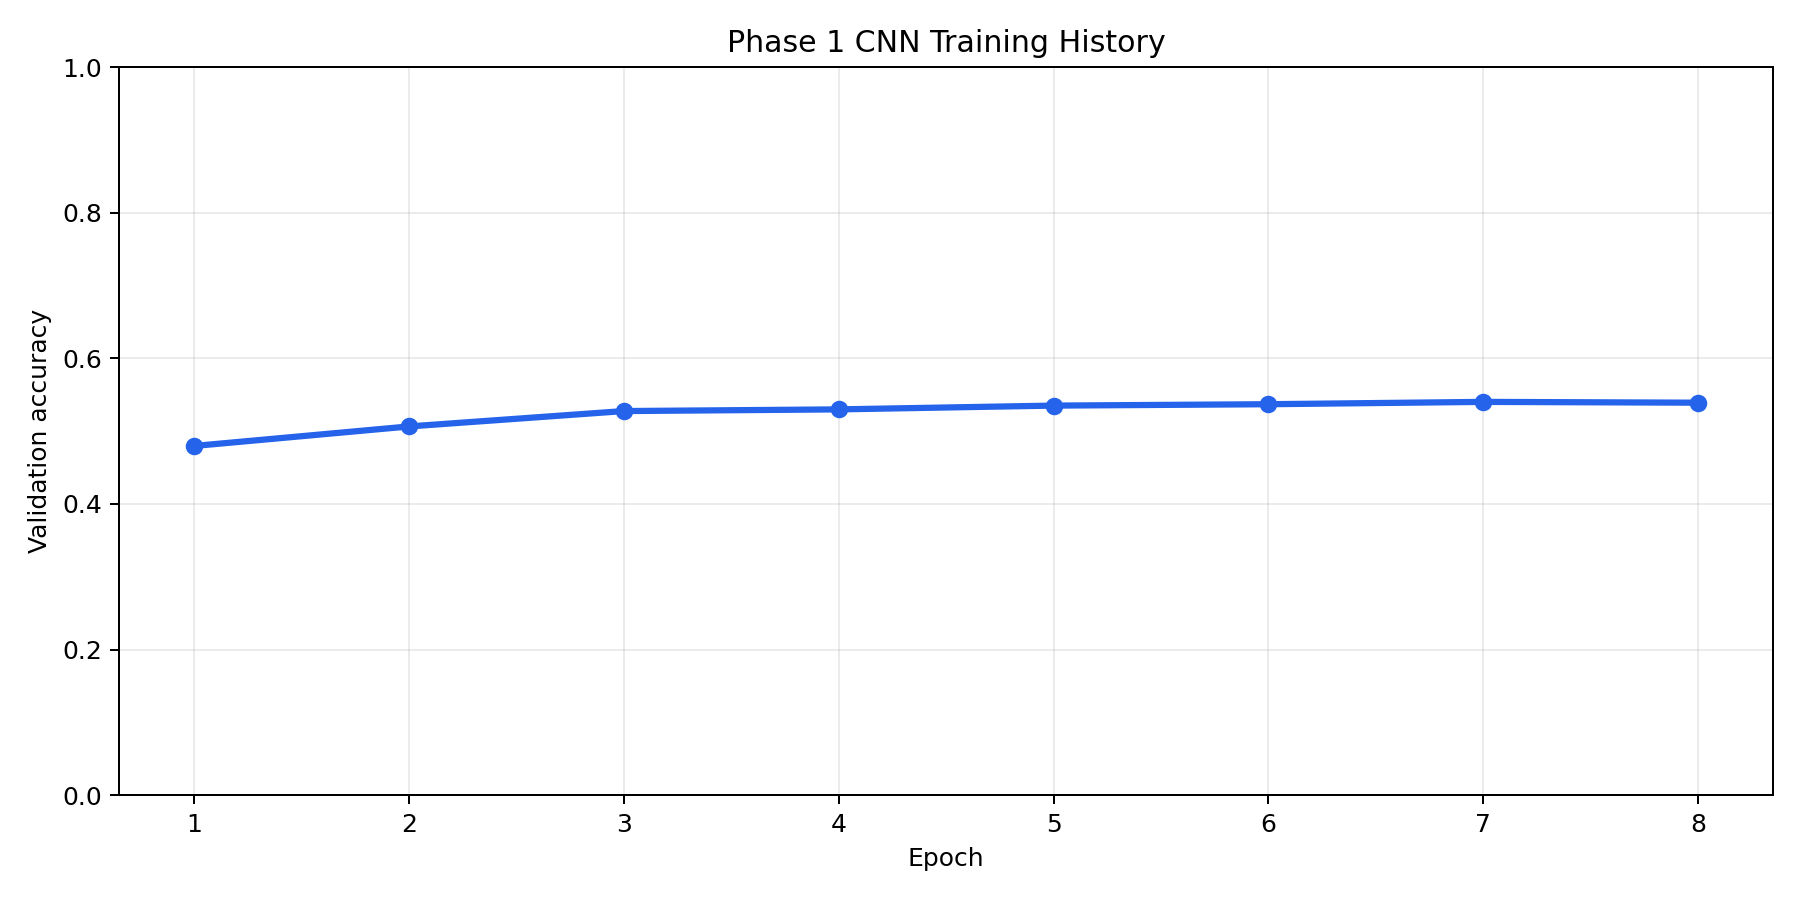
\includegraphics[width=0.9\textwidth]{artifacts/phase1-training-history.png}
\caption{Phase 1 CNN validation accuracy history.}
\label{fig:traininghistory}
\end{figure}

\section{Phase 2 Communication Results}
The Phase 2 receiver shows a clear operating transition as SNR increases.
At low SNR, the constellation decision is uncertain and the selected
demodulator frequently does not match the transmitter. At higher SNR, the
decision becomes reliable and the recovered information quality improves.

\begin{table}[H]
\centering
\caption{Selected Phase 2 measured results.}
\begin{tabular}{c c c c c c}
\hline
\textbf{SNR} & \textbf{BER} & \textbf{SER} & \textbf{Decision} &
\textbf{Packet} & \textbf{Throughput}\\
\hline
10 dB & 4.69\% & 6.94\% & 99.5\% & 49.0\% & 1.225\\
12 dB & 1.85\% & 3.05\% & 100.0\% & 54.5\% & 1.363\\
16 dB & 0.095\% & 0.172\% & 100.0\% & 75.5\% & 1.888\\
\hline
\end{tabular}
\end{table}

\begin{figure}[H]
\centering
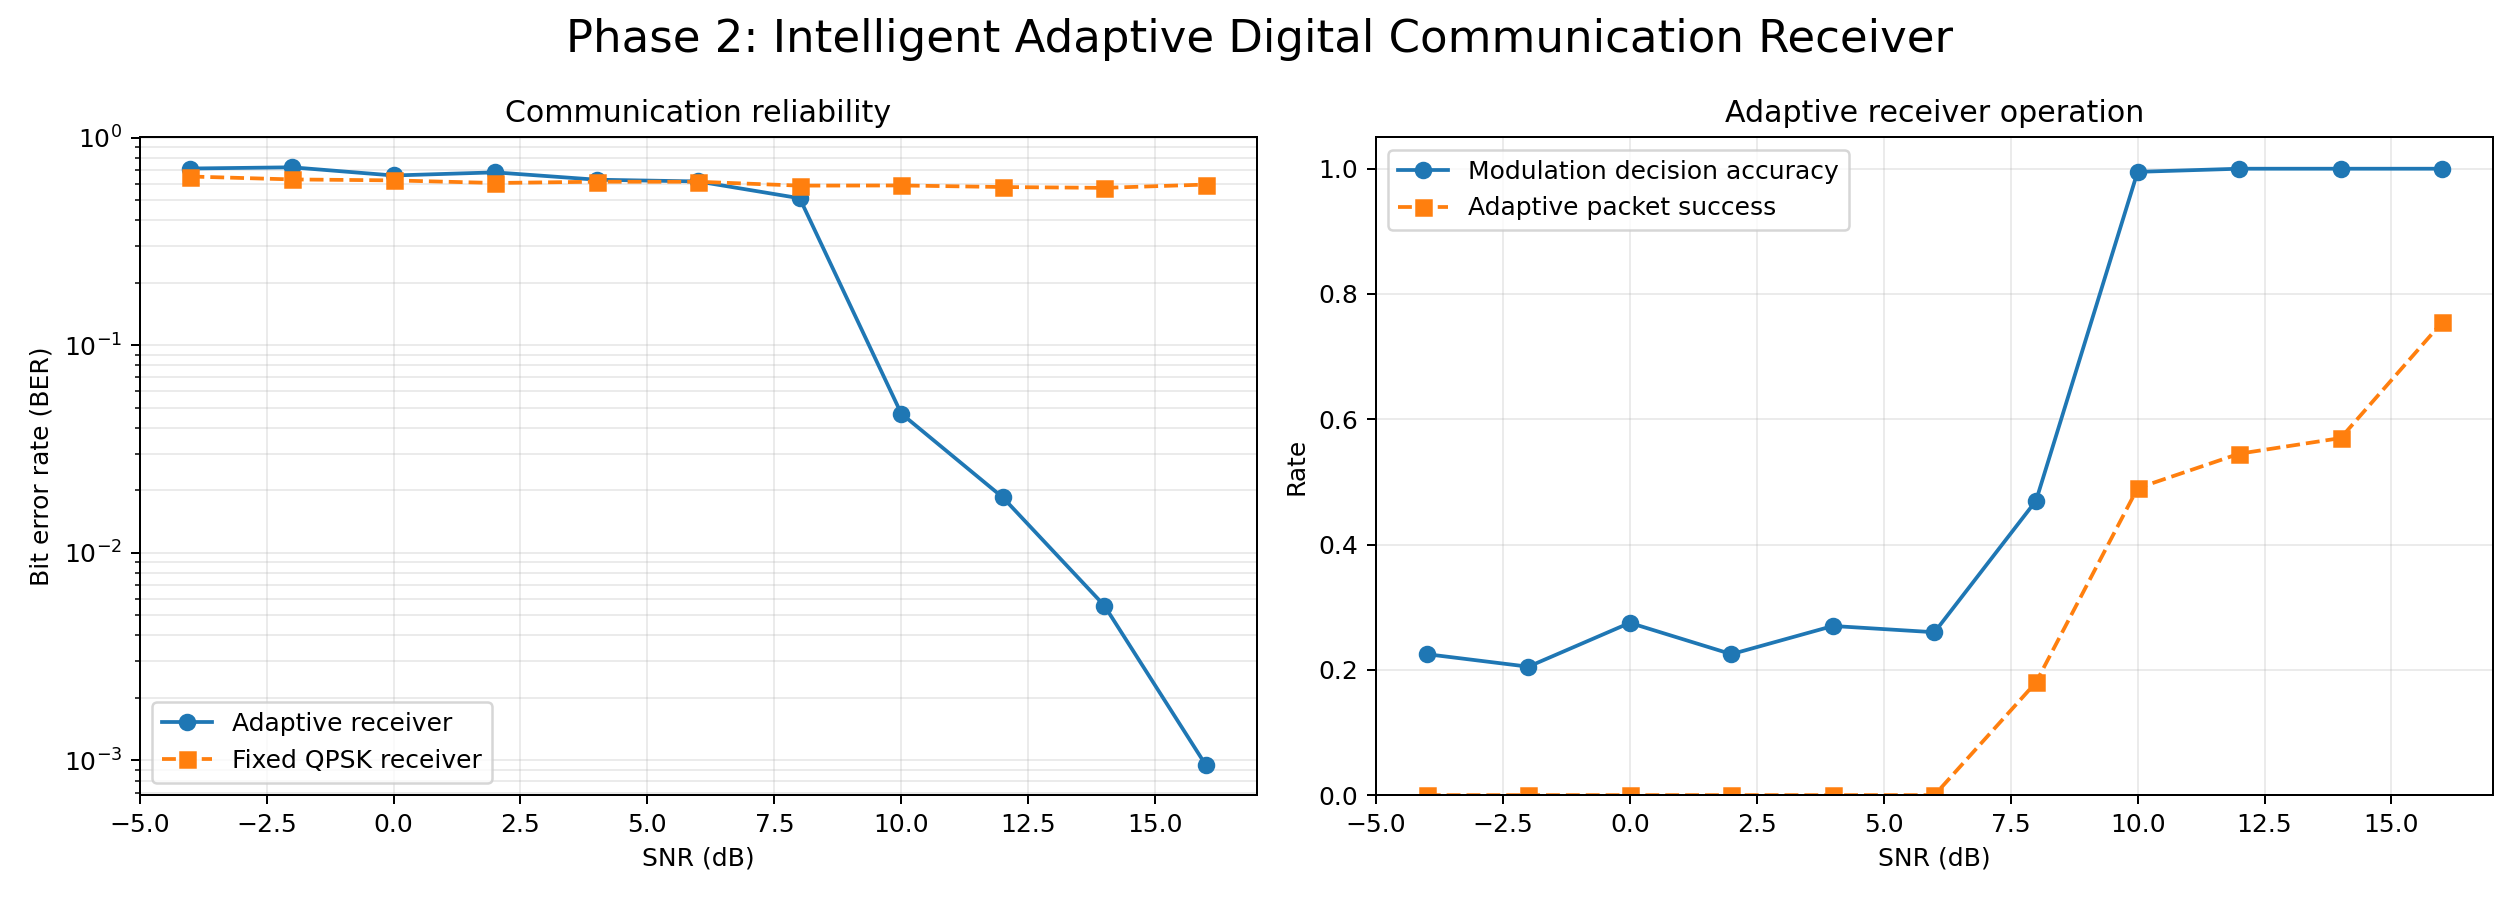
\includegraphics[width=\textwidth]{artifacts/phase2-link-results.png}
\caption{Phase 2 BER, SER, decision accuracy, packet success, and throughput.}
\label{fig:phase2result}
\end{figure}

\section{Parameter Records}
\begin{figure}[H]
\centering
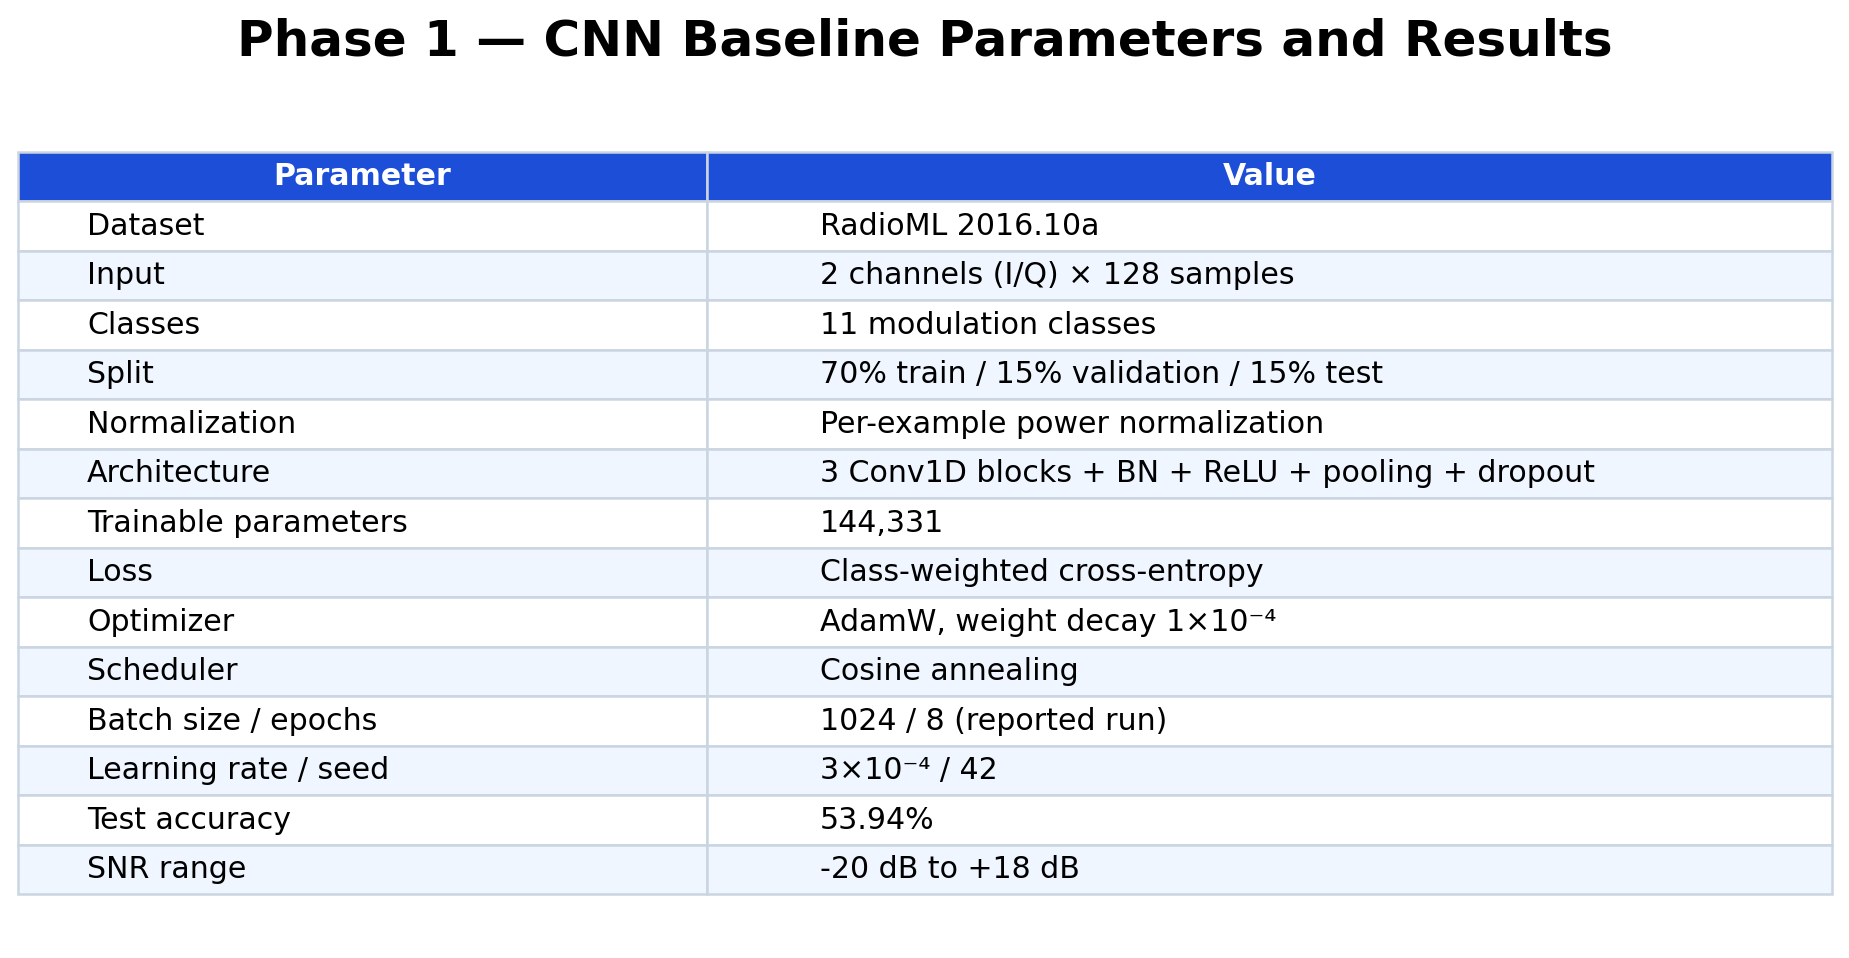
\includegraphics[width=\textwidth]{artifacts/phase1-parameters-results.png}
\caption{Phase 1 model and training parameters.}
\label{fig:phase1parameters}
\end{figure}

\begin{figure}[H]
\centering
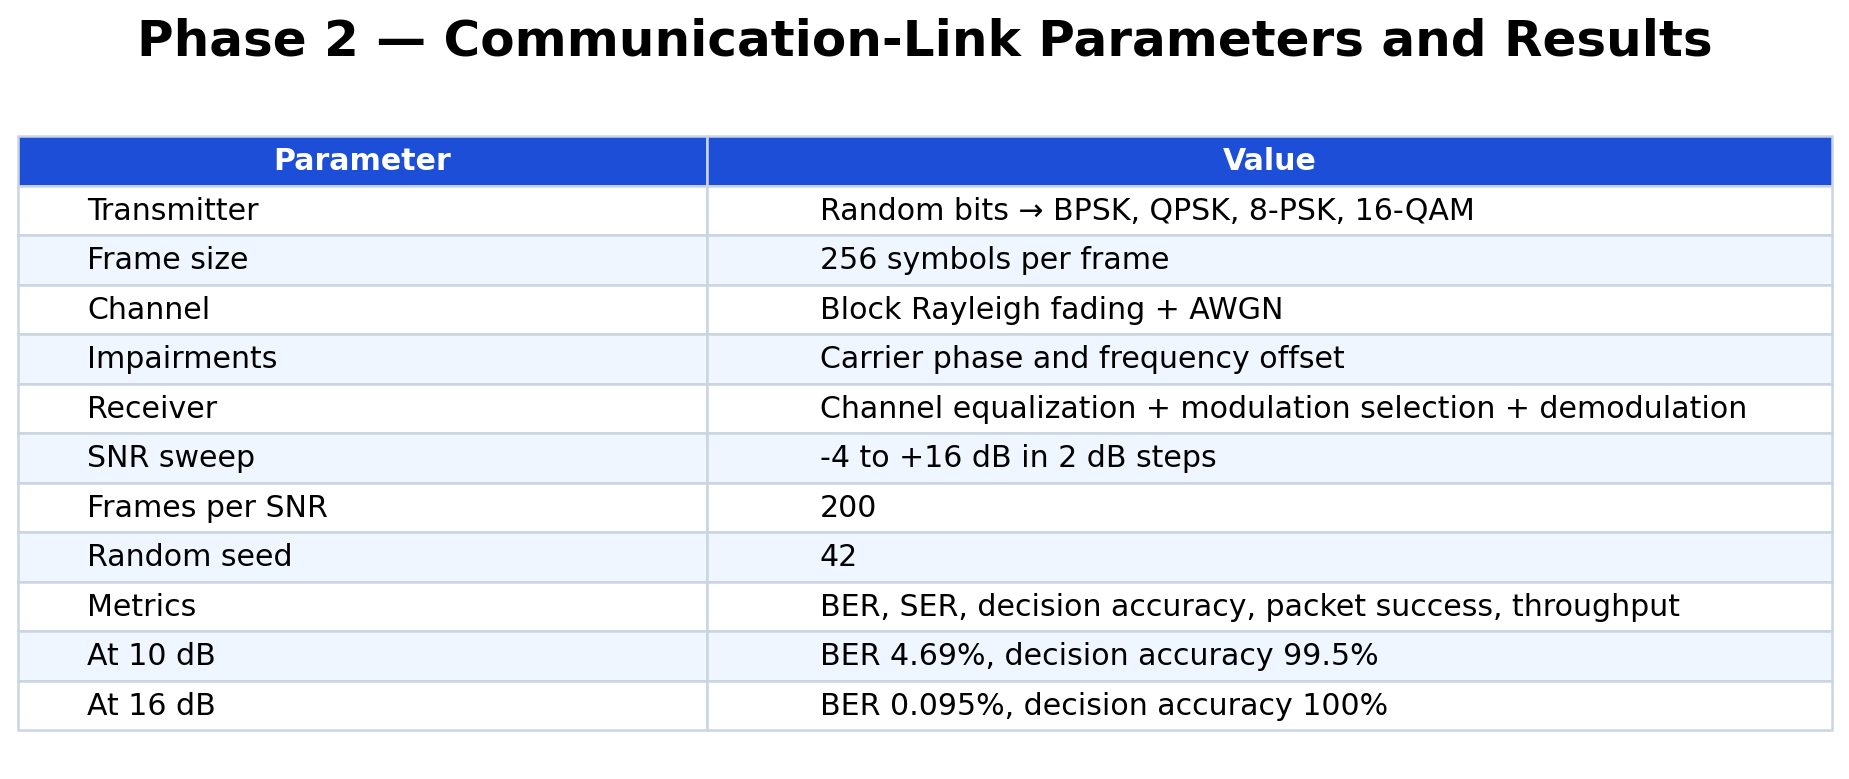
\includegraphics[width=\textwidth]{artifacts/phase2-parameters-results.png}
\caption{Phase 2 communication-link parameters and results.}
\label{fig:phase2parameters}
\end{figure}

\section{Phase 1 and Phase 2 Comparison}
\begin{table}[H]
\centering
\caption{Technical comparison between project phases.}
\begin{tabular}{p{5cm} p{4cm} p{4cm}}
\hline
\textbf{Aspect} & \textbf{Phase 1} & \textbf{Phase 2}\\
\hline
Main goal & Modulation classification & Adaptive communication receiver\\
Input & Fixed labeled RadioML samples & Generated information frames\\
Output & Class label & Recovered bits and link metrics\\
Channel & Dataset-provided conditions & AWGN, Rayleigh, offsets\\
Receiver action & No demodulator control & Automatic demodulator selection\\
Metrics & Accuracy and confusion & BER, SER, packet success, throughput\\
Representative result & 53.94\% test accuracy & 0.095\% BER at 16 dB\\
\hline
\end{tabular}
\end{table}

\begin{figure}[H]
\centering
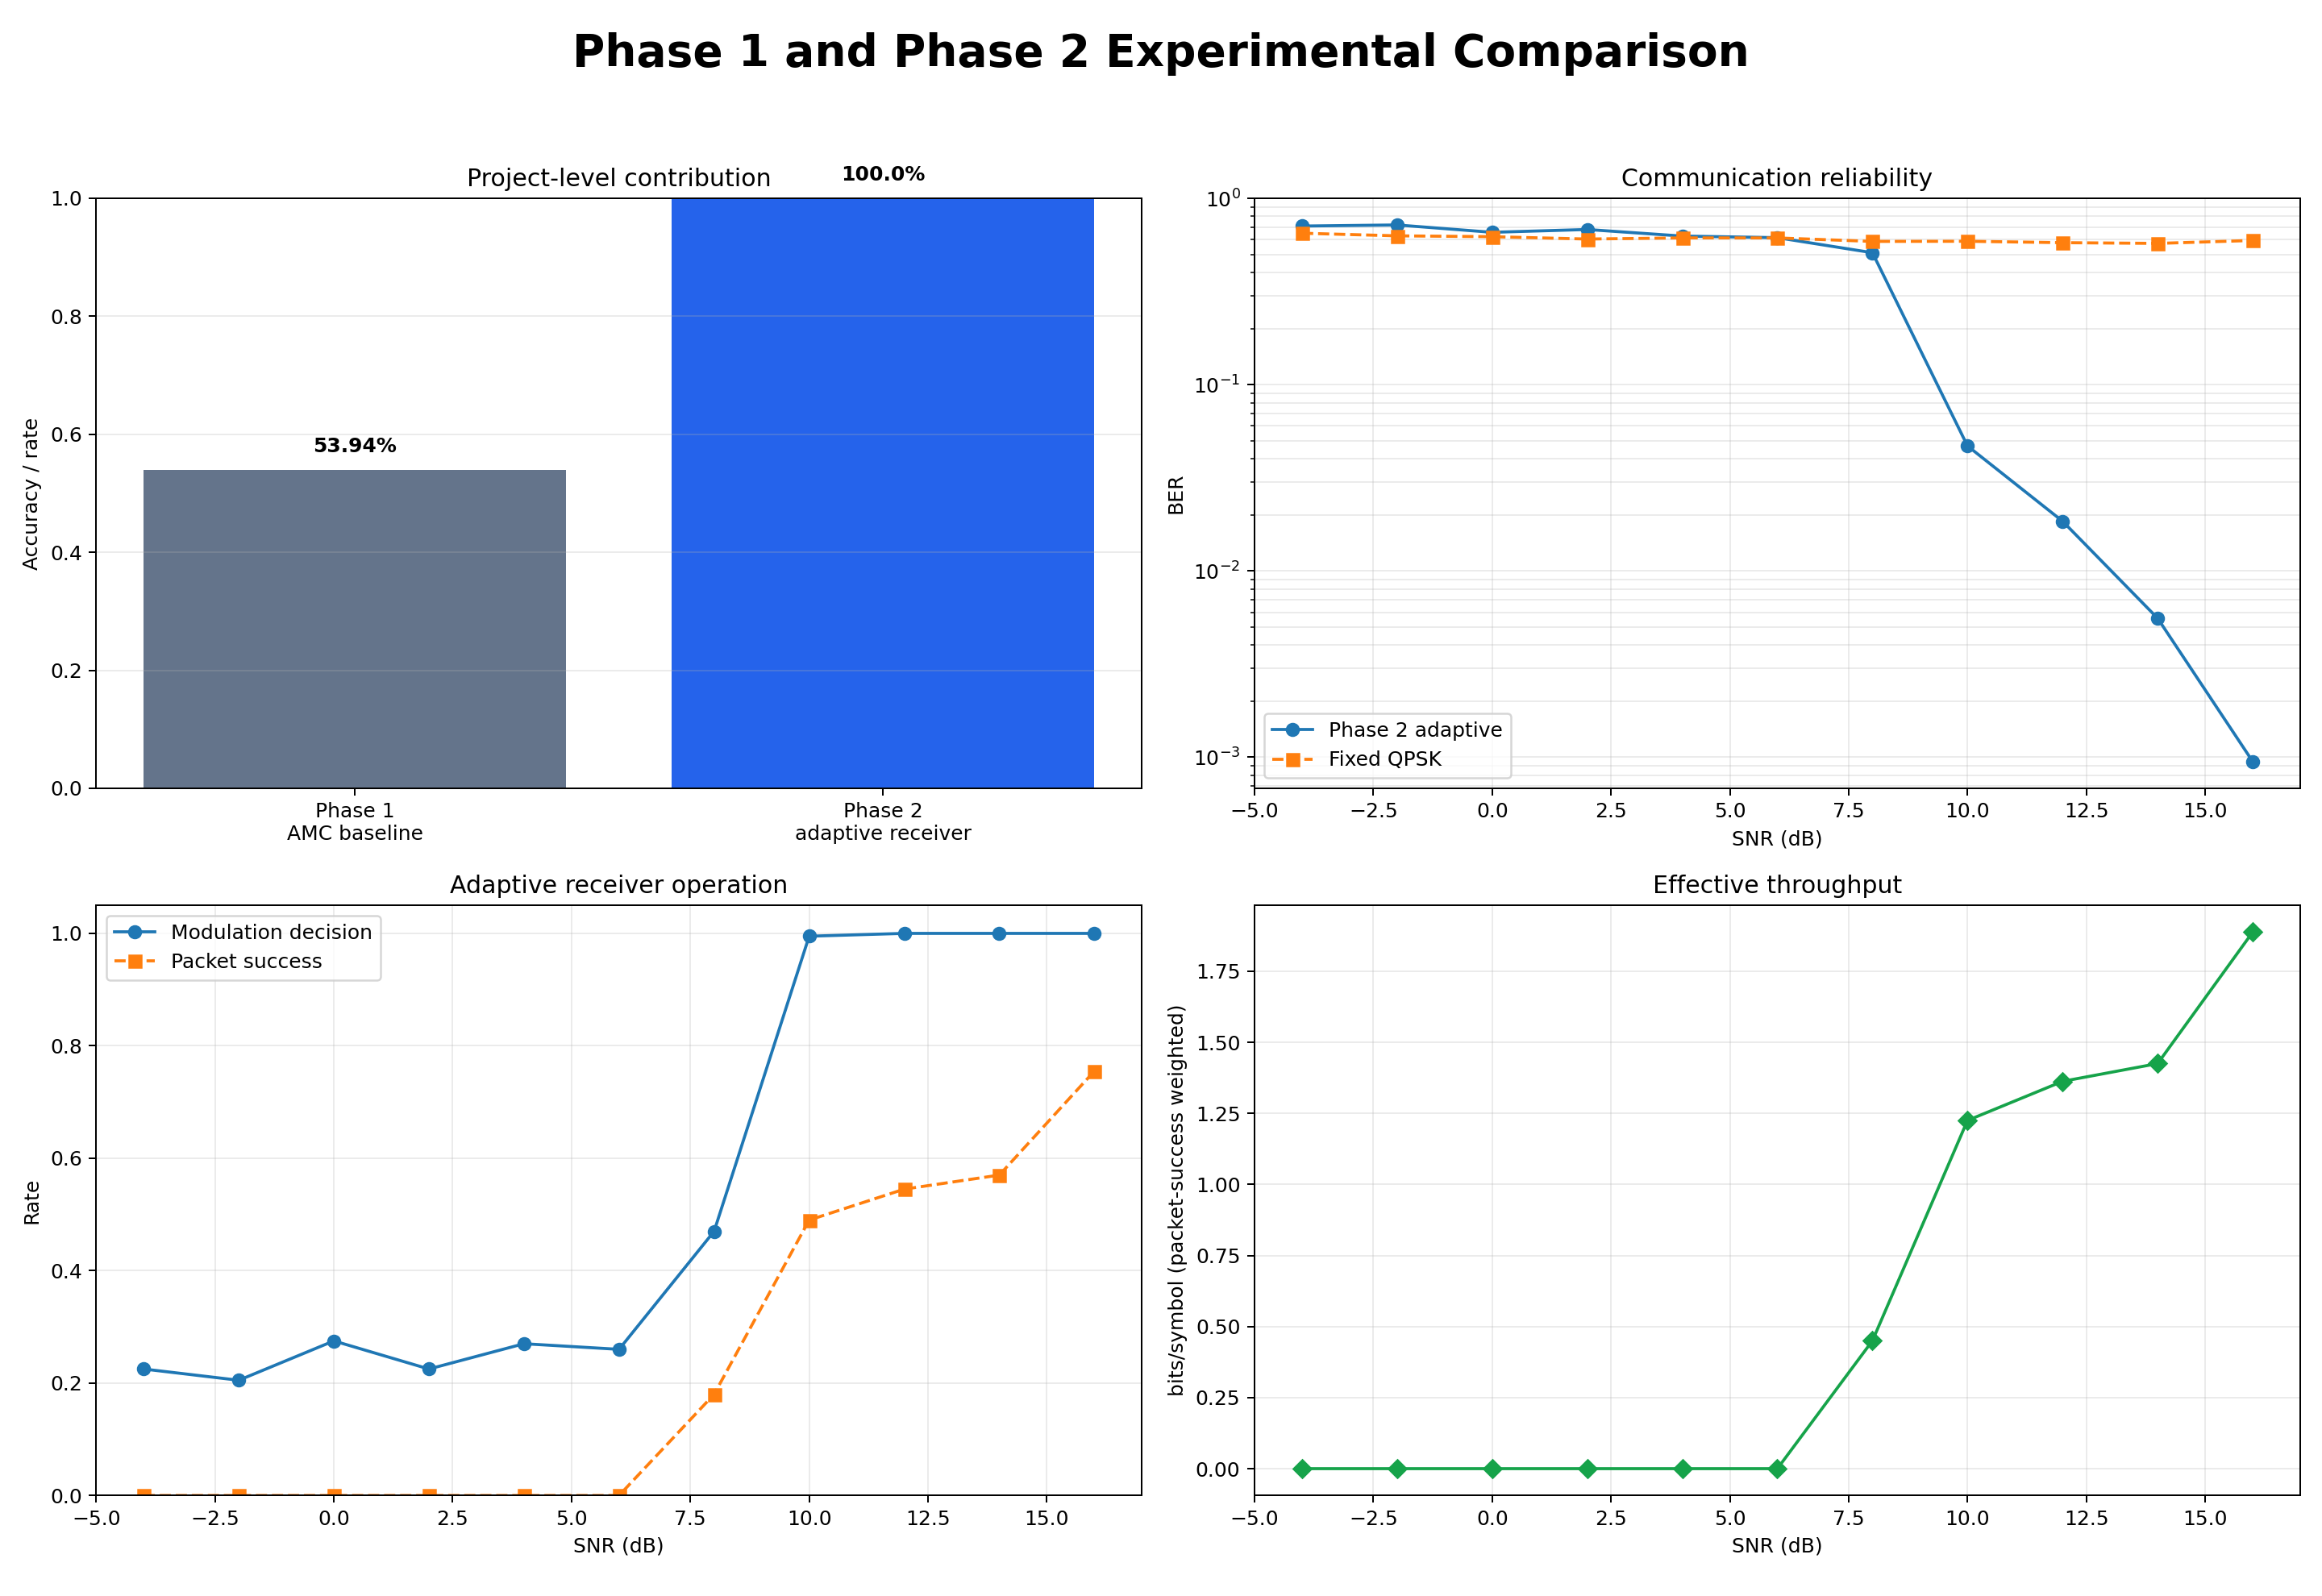
\includegraphics[width=\textwidth]{artifacts/final-phase1-phase2-comparison.png}
\caption{Consolidated Phase 1 and Phase 2 comparison.}
\label{fig:comparison}
\end{figure}

\section{Communication Interpretation}
The Phase 2 experiment demonstrates why recognition accuracy alone is not
sufficient for a communication project. A wrong modulation decision changes
the demodulator and can cause an entire packet to fail. At 16 dB, all tested
modulation decisions were correct in the reported run and the BER was below
one tenth of one percent. At low SNR, the receiver exposes the operating
limit instead of hiding it behind a single average accuracy value.
